\documentclass[letterpaper, reqno,11pt]{article}
\usepackage[margin=1.0in]{geometry}
\usepackage{color,latexsym,amsmath,amssymb,graphicx,float,listings,tikz}
\usepackage{hyperref}

\hypersetup{
colorlinks=true,
linkcolor=magenta,
filecolor=magenta,
urlcolor=cyan,
}

\graphicspath{ {images/} }

\tikzstyle{vertex}=[shape=circle, minimum size=2mm, fill, draw, inner sep=0]

\begin{document}
\pagenumbering{arabic}
\title{Math 443 Homework 5}
\date{01/03/23}
\author{Xander Naumenko}
\maketitle

{\medskip\noindent\bf Question 1.} Let $k$ be a positive integer, and let $A_1,A_2$ be two copies of $K_{k+1}$. Let $G_k$ be created by taking a new vertex, $v$, and connecting it to $k$ vertices in each of $A_1,A_2$. Clearly $\kappa(G_k)=1$ since if $v$ is removed $G_k$ gets separated into $A_1,A_2$ as components. To see that $\lambda(G_k)\leq k$, note that by removing all edges between $v$ and $A_1$ results in a disconnect graph, which is an edge set of size $k$. 

To see why this is a minimum edge cut, let $E\subset E(G_k)$ s.t. $|E|<k$ (since $E$ is an edge set the $\left|  \right| $ syntax denotes size of set, not number of vertices). Then $E$ couldn't have removed all the edges between $A_1$ and $v$, since there are $k$ edges between them. By symmetry the same applies for $A_2$ and $v$. $A_1-E$ and $A_2-E$ are still connected since they are both copies of $K_k$, so the total graph is also connected. Thus $\lambda(G_k)=k$ and $\kappa(G_k)=1$ as required. 

{\medskip\noindent\bf Question 2a.} The statement is true. Let $E$ be a separating edge set of $G$, and let $A$ be a smallest resulting component of $G-E$. Clearly $|A|\leq \frac{n}{2}$ since it the smaller of at least two components whose total vertices is $n$. Note that $| |A| |\leq K_{|A|}=|A|(|A|-1)$. Also note that the total number of edges of the vertices of $A$ in $G$ is $|A|\cdot \delta(G)$. The difference between these numbers is at least the number of vertices taken away by $E$, i.e. $|E|\geq |A| \delta(G)-|A|(|A|-1)=|A|\left( \delta(G)-|A|+1 \right) $. This is a downward parabola, so from calculus its minimum must lie on one of the two endpoints, i.e. $|A|=1$ or $|A|=\frac{n}{2}$. These two values are: 
\[
|E|\geq \delta(G)-1+1=\delta(G)
.\]
\[
|E|\geq \frac{n}{2}(\delta(G)-\frac{n}{2}+1)\geq \delta(G)
.\]
We conclude that $\lambda(G)\geq \delta(G)$. In class we also proved that $\lambda(G)\leq \delta(G)$, so these two inequalities together tell us that $\lambda(G)=\delta(G)$ as required. $\square$

{\medskip\noindent\bf Question 2b.} The statement is false. As a counterexample let $k\geq 3$ and consider two copies of $K_k$, $A_1,A_2$. Form $G$ by adding two vertices $v_1,v_2$ connected to all vertices in $A_1,A_2$. Each vertex in $A_1,A_2$ has $k-1$ neighbors from the complete graph as well as $v_1,v_2$ for a total of $k-1+2=k+1$. $v_1,v_2$ each have $2k$ neighbors since their connected to each vertex in $A_1,A_2$. The total vertices is $2k+2$, so $\delta(G)=k+1\geq \frac{|G|}{2}$. We can disconnect the graph by removing $v_1,v_2$, so $\kappa=2$ (it clearly can't be less than that). Let $E$ be an edge set with $|E|\leq 2$. $A_1$ remain connected in $G-E$ since they are $k\geq 3$ complete, and there is at least one edge from $A_1$ to $v_1$ and $v_2$ in $G-E$, since there were at least $3$ edges before and $E$ removed at most 2. By symmetry the same is true for $A_2$, so all 4 of $A_1,A_2,v_1,v_2$ are internally connected and connected together. Thus $E$ is not an edge cut, so $\lambda(G)>2$ and $\lambda(G)\neq \kappa(G)$.  

{\medskip\noindent\bf Question 3.} The statement is not true. Consider the following graph $G$: 

\begin{center}
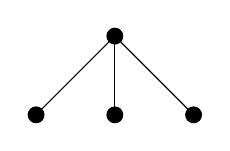
\begin{tikzpicture}
\draw (0,0)node[vertex]{};
\draw (1,0)node[vertex]{};
\draw (2,0)node[vertex]{};
\draw (1,1)node[vertex]{};
\draw (0,0)--(1,1);
\draw (1,0)--(1,1);
\draw (2,0)--(1,1);
\end{tikzpicture}
\end{center}

The three groups are three copies of $K_2$, and they are each connected to each other since they each share a vertex, so this is $\mathcal{G}$: 

\begin{center}
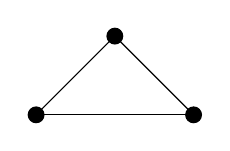
\begin{tikzpicture}
\draw (0,0)node[vertex]{};
\draw (2,0)node[vertex]{};
\draw (1,1)node[vertex]{};
\draw (0,0)--(1,1);
\draw (2,0)--(1,1);
\draw (0,0)--(2,0);
\end{tikzpicture}
\end{center}

This obviously isn't a tree since it contains a cycle, so we're done and the statement is false. 

{\medskip\noindent\bf Question 4a.} The statement is true. Let $v\in G[\mathcal{E}]$. Let $x,y\in G[\mathcal{E}]-v$. Let $C$ be a cycle in $G[\mathcal E]$ containing $x,y$ (this exists since you can choose any two edges attached to $x,y$ and they're guaranteed to share a cycle). Let $P$ be a path along $C$ that doesn't include $v$, since there are two options (each way around $C$) this will always exist. Then $x,y$ are connected in $G[\mathcal{E}]-v$ through $P$. This works for any $v$, so there are no cut vertices in $G[\mathcal{E}]$ so it is nonseparable. $\square$

%\includegraphics[width=0.015\textwidth]{Epsilon}

{\medskip\noindent\bf Question 4b.} The statement is true. From the definition of $G[\mathcal E]$, $E(G[\mathcal E])\subset E(G)$. The vertex set of $G[\mathcal E]$ is the vertex set of all endpoints of $\mathcal E$ in $G$, since these are the vertices that don't become isolated vertices when $E(G)-\mathcal E$ are removed from $G$. This is exactly the definition of an induced subgraph though, so $G[\mathcal E]\leq G$. $\square$

{\medskip\noindent\bf Question 4c.} The statement is true. We will use proof by contradiction. From part a $G[\mathcal E]$ is nonseparable, so the only way $G[\mathcal E]$ could not be a block is if it isn't maximal. By way of contradiction suppose that $\exists B\subset G, v\in G, v\notin G[\mathcal E]$ s.t. $B$ is nonseparable and $V(G[\mathcal E])\subset V(B), v\in B,$. It is asserted that there exists paths $P_1,P_2$ from $v$ to $G[\mathcal E]$ in $B$ with the endpoints of $u_1,u_2\in G[\mathcal E], u_1\neq u_2$. At least one path $P_1$ must exist for $v$ and $G[\mathcal E]$ to be connected, and since removing $u_1$ shouldn't disconnect $G[\mathcal E]+v$ a second path must exist with a different endpoint in $G[\mathcal E]$. Choose $P_1,P_2$ in such a way that $u_1,u_2$ are their only member in $G[\mathcal E]$. Consider the first common ancestor between $P_1$ and $P_2$ starting from $u_1,u_2$, call it $x$. $G[\mathcal E]$ is connected so there exists a path in it between $u_1$ and $u_2$, call it $P_3$. Then $u_1P_3u_2P_1xP_2u_1$ is a cycle in $G$ containing an edges not in $G[\mathcal E]$, namely the edges of $P_1,P_2$ before $x$. This is impossible since we assumed $G[\mathcal E]$ was formed by the entire equivalence class, so it must be that $G[\mathcal E]$ is a block of $G$. $\square$

{\medskip\noindent\bf Question 4d.} The statement is false. Consider the extr

\end{document}
